% Fig. 3  Round 6: K1 first run vs. K3 post-hoc (single column, drawn at 3.45 in).
% Data: ../data/round6_k1_k3.csv, extracted from evaluation/v3/results/final6_K1_first_and_only.json
% and final6_K3_posthoc_not_heldout.json (commit b11793b; K1 recorded in 7e30dc4, K3 in a63cec1).
\documentclass[border=2pt]{standalone}
% Shared settings for all InsightFlow AI figures (Times, grayscale, sized for IEEE print).
\usepackage[T1]{fontenc}
\usepackage{mathptmx}
\usepackage{tikz}
\usetikzlibrary{positioning,arrows.meta,calc,fit,patterns,shapes.geometric}
\tikzset{
  >={Stealth[length=4pt,width=3.5pt]},
  stage/.style={draw,rounded corners=1.5pt,fill=gray!8,align=center,inner sep=2.5pt,font=\fontsize{7.5}{8.6}\selectfont},
  ext/.style={draw,dashed,rounded corners=1.5pt,align=center,inner sep=2.5pt,font=\fontsize{7.5}{8.6}\selectfont},
  note/.style={align=left,font=\fontsize{7}{8}\selectfont},
  flow/.style={->,thick},
  dflow/.style={->,dashed},
  every node/.append style={execute at begin node={\hyphenpenalty=10000\exhyphenpenalty=10000}},
}

\usepackage{pgfplots}
\pgfplotsset{compat=1.17}
\begin{document}
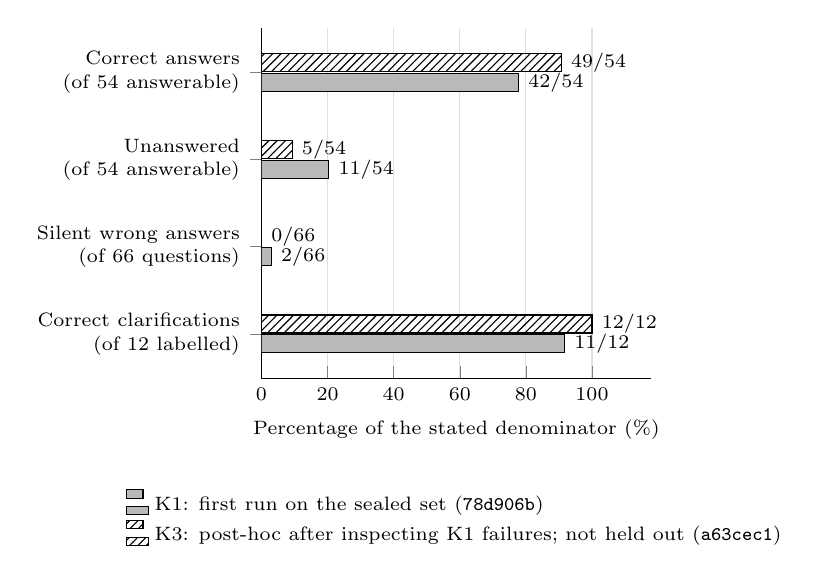
\begin{tikzpicture}
\begin{axis}[
  width=1.95in, height=1.75in, scale only axis=true,
  xbar=0.6pt, bar width=6.5pt,
  xmin=0, xmax=118, xtick={0,20,40,60,80,100},
  xlabel={Percentage of the stated denominator (\%)},
  xlabel style={font=\fontsize{7.5}{8.6}\selectfont},
  ytick=data, y dir=reverse,
  symbolic y coords={corr,unans,silent,clar},
  yticklabels={{Correct answers\\(of 54 answerable)},{Unanswered\\(of 54 answerable)},{Silent wrong answers\\(of 66 questions)},{Correct clarifications\\(of 12 labelled)}},
  yticklabel style={align=right,font=\fontsize{7.5}{8.6}\selectfont},
  xticklabel style={font=\fontsize{7.5}{8.6}\selectfont},
  enlarge y limits=0.17, axis x line*=bottom, axis y line*=left,
  xmajorgrids, grid style={gray!25},
  nodes near coords, nodes near coords style={font=\fontsize{7}{8}\selectfont,anchor=west},
  point meta=explicit symbolic,
  legend style={font=\fontsize{7}{8}\selectfont,at={(0.5,-0.30)},anchor=north,legend columns=1,draw=none,cells={anchor=west}},
  reverse legend=false,
]
\addplot[draw=black,fill=gray!55] coordinates {(77.8,corr)[42/54] (20.4,unans)[11/54] (3.0,silent)[2/66] (91.7,clar)[11/12]};
\addplot[draw=black,pattern=north east lines] coordinates {(90.7,corr)[49/54] (9.3,unans)[5/54] (0.0,silent)[0/66] (100.0,clar)[12/12]};
\legend{{K1: first run on the sealed set (\texttt{78d906b})},{K3: post-hoc after inspecting K1 failures; not held out (\texttt{a63cec1})}}
\end{axis}
\end{tikzpicture}
\end{document}
